%\documentclass[aspectratio=43]{beamer}
\documentclass[8pt, compress]{beamer}
\usepackage[utf8]{inputenc}
\usepackage[T1]{fontenc}
\usepackage[absolute,overlay]{textpos}
\usepackage{graphicx}
\usepackage{subfig}
\usepackage{framed}
\usepackage{color}
\usepackage{transparent}

%\geometry{paperwidth=175mm,paperheight=108.75mm}
\geometry{paperwidth=155mm,paperheight=116mm}

\usepackage{array}
\usepackage{times}
\usepackage{palatino}
\usepackage{mathtools}
\usepackage{verbatim}
%\usepackage{RT_woutmeshate}
\usepackage{xmpmulti}

\newcommand{\pdv}[2]{\frac{\partial{#1}}{\partial{#2}}}
\newcommand{\vect}[1]{\boldsymbol{#1}}
\newcommand{\matr}[1]{\mathbf{#1}}
\newcommand{\dI}{\text{d}}
\newcommand{\odv}[2]{\frac{\dI #1}{\dI #2}}
\newcommand{\ddv}[2]{\odv{#1}{#2}}
\newcommand{\mfpe}{\lambda_e}
\newcommand{\mfpei}{\lambda_{ei}}
\newcommand{\Zbar}{Z}
\newcommand{\nue}{\nu_{e}}
\newcommand{\nuei}{\nu_{ei}}
\newcommand{\nuscat}{\nu_{scat}}
\newcommand{\vmag}{v}
\newcommand{\vth}{v_{th}}
\newcommand{\vtwoh}{v_{2 th}}
\newcommand{\vn}{\vect{n}}
\newcommand{\E}{\vect{E}}
\newcommand{\B}{\vect{B}}
\newcommand{\omegaB}{\vect{\omega}_{B}}
\newcommand{\Ez}{E_z}
\newcommand{\qe}{q_e}
\newcommand{\me}{m_e}
\newcommand{\Te}{T_e}
\newcommand{\Ti}{T_i}
\newcommand{\ed}{n_e}
\newcommand{\kB}{k_B}
\newcommand{\fM}{f_M}
\newcommand{\fzero}{f_0}
\newcommand{\vfzero}{\vect{f_0}}
\newcommand{\fone}{{\vect{f_1}}}
\newcommand{\fonez}{f_{1_z}}
\newcommand{\vv}{\vect{v}}
\newcommand{\vvb}{\tilde{\vect{v}}}
\newcommand{\gv}{\nabla_{\vv}}
\newcommand{\gvb}{\nabla_{\vvb}}
\newcommand{\gx}{\nabla_{\vect{x}}}
\newcommand{\ft}{f}
\newcommand{\lnc}{\text{ln}\Lambda}
\newcommand{\Iohm}{\matr{J}_{Ohm}}

\newcommand{\vsp}[1]{\vspace{#1mm}}
\newcommand{\colorimportant}[1]{ {\color{purple} #1} }

\definecolor{shadecolor}{rgb}{1,0.8,0.3}
\colorlet{shadecolor}{yellow!30}

\usetheme{llnl}
\newtheorem{conjecture}[theorem]{Conjecture}

\newcommand{\ba}{{\bf a}}
\newcommand{\bb}{{\bm b}}
\newcommand{\bc}{{\bm c}}
\newcommand{\bd}{{\bm d}}
\newcommand{\be}{{\bm e}}
\newcommand{\bg}{{\bm g}}
\newcommand{\bh}{{\bm h}}
\newcommand{\bi}{{\bm i}}
\newcommand{\bj}{{\bm j}}
\newcommand{\bk}{{\bm k}}
\newcommand{\bl}{{\bm l}}
\newcommand{\bn}{{\bm n}}
\newcommand{\bo}{{\bm o}}
\newcommand{\bp}{{\bm p}}
\newcommand{\bq}{{\bm q}}
\newcommand{\br}{{\bm r}}
\newcommand{\bs}{{\bm s}}
\newcommand{\bt}{{\bm t}}
\newcommand{\bu}{{\bf u}}
\newcommand{\bv}{{\bf v}}
\newcommand{\bw}{{\bm w}}
\newcommand{\bx}{{\bf x}}
\newcommand{\by}{{\bf y}}
\newcommand{\bz}{{\bm z}}


\newcommand{\bfz}{{\bf 0}}

\newcommand{\cA}{\mathcal{A}}
\newcommand{\cB}{\mathcal{B}}
\newcommand{\cC}{\mathcal{C}}
\newcommand{\cD}{\mathcal{D}}
\newcommand{\cE}{\mathcal{E}}
\newcommand{\cF}{\mathcal{F}}
\newcommand{\cG}{\mathcal{G}}
\newcommand{\cH}{\mathcal{H}}
\newcommand{\cI}{\mathcal{I}}
\newcommand{\cJ}{\mathcal{J}}
\newcommand{\cK}{\mathcal{K}}
%\newcommand{\cL}{\mathcal{L}}
\newcommand{\cL}{L}
\newcommand{\cM}{\mathcal{M}}
\newcommand{\cN}{\mathcal{N}}
\newcommand{\cO}{\mathcal{O}}
\newcommand{\cP}{\mathcal{P}}
\newcommand{\cQ}{\mathcal{Q}}
\newcommand{\cR}{\mathcal{R}}
\newcommand{\cS}{\mathcal{S}}
\newcommand{\cT}{\mathcal{T}}
\newcommand{\cU}{\mathcal{U}}
\newcommand{\cV}{\mathcal{V}}
\newcommand{\cW}{\mathcal{W}}
\newcommand{\cX}{\mathcal{X}}
\newcommand{\cY}{\mathcal{W}}
\newcommand{\cZ}{\mathcal{Z}}

\definecolor{green}{rgb}{0.13,.54,0.13}
\newcommand{\red}[1]{\textcolor{red}{#1}}
\newcommand{\green}[1]{\textcolor{green}{#1}}
\newcommand{\blue}[1]{\textcolor{blue}{#1}}

\title{{\Huge Multi-dimensional High-Order FEM Methods for Electron Kinetics in ALE Hydrodynamics}}
\date{{\Huge February 25 - March 1, 2019}}
\author[Last Name]{{\Huge Milan Holec, Ben S. Southworth}}
\IMNumber{{\Huge LLNL-PRES-768124}}
\conference{{\huge SIAM Conference on Computational Science and Engineering (CSE19)}}
\location{{\Huge Spokane, Washington, USA}}

\begin{document}
\begin{frame}
 \titlepage
\end{frame}

\begin{frame}
  \tableofcontents
\end{frame}

\section{Motivation - Nonlocal Magneto-Hydrodynamic model (Nonlocal-MHD)}

\begin{comment} % 2T MHD
\begin{frame}
\begin{center}
{\huge Classical MHD}  

\begin{eqnarray}
  \text{HYDRODYNAMICS} && 
  local \rightarrow \vect{q}_e = - \kappa_{SH} \Te^{2.5} \nabla \Te \nonumber \\
  && \nonumber \\
  \frac{\dI \rho}{\dI t} &=& - \rho\nabla\cdot\vect{u} , 
  \nonumber\\ 
  \rho\, \frac{\dI \vect{u}}{\dI t} &=& - \nabla (p_i + p_e) 
  + \frac{c}{4\pi}\nabla\times\vect{B}\times \vect{B}, 
  \nonumber\\   
  \rho \left(\frac{\partial \varepsilon_i}{\partial T_i}\frac{\dI T_i}{\dI t} 
  +\frac{\partial \varepsilon_i}{\partial \rho}\frac{\dI \rho}{\dI t}\right)
  &=& 
  - p_i\nabla\cdot\vect{u} - G(T_i - T_e) , 
  \nonumber\\
  \rho \left(\frac{\partial \varepsilon_e}{\partial T_e}\frac{\dI T_e}{\dI t}
  +\frac{\partial \varepsilon_e}{\partial \rho}\frac{\dI \rho}{\dI t}\right)
  %+ \frac{\dI \epsilon_R}{\dI t} 
  &=& 
  - p_e \nabla\cdot\vect{u} 
  + \nabla\cdot\left(\kappa_{SH} \Te^{2.5} \nabla \Te \right) 
  + \sigma \E\cdot\E
  + G(T_i - T_e) + Q_{\text{IB}}(\vect{E}_L) , 
  \nonumber \\
  && \nonumber \\
  && \nonumber \\
  \text{MAXWELL EQUATIONS} && 
  resistive\rightarrow\vect{j} = \sigma \E \nonumber \\
  && \nonumber \\
  \nabla\times\vect{E} &=& -\frac{1}{c}\frac{\dI \vect{B}}{\dI t} ,
  %\quad\qquad (\text{life of magnetic field}~\vect{B}~\text{in the fluid frame})
  \nonumber \\
  \nabla\times\vect{B} &=& \frac{4\pi}{c}
  \sigma \E ,%\quad~~~ (\vect{j} \text{ depends on }f\text{ and }\vect{E}\text{ from the nonlocal model}) 
  \nonumber \\
  && \nonumber \\
  \hline \nonumber \\
  %&& \nonumber \\
  \text{KINETICS OF ELECTRONS} && Landau-Fokker-Planck \nonumber \\
  && \nonumber \\
  \pdv{f}{t} + \vect{v}\cdot\nabla f +
  \left( \vect{E} + \vect{v}\times\vect{B}\right)\cdot\nabla_{\vect{v}} f
  &=& 
  \Gamma\int \gv\gv(\vv - \vvb) \cdot \left(
  \ft\, \gvb \ft - \ft\, \gv \ft \right)\, \dI\vvb
  + \frac{\nuei}{2} \frac{\partial^2 f}{\partial \Omega^2} .
  \nonumber
\end{eqnarray}
%\let\thefootnote\relax\footnote{Spitzer and Harm, \textit{Phys. Rev.}, (1953).}
\end{center}
\end{frame}

\begin{frame}
\begin{center}
{\huge Nonlocal-MHD}  

\begin{eqnarray}
  \text{HYDRODYNAMICS} && \text{4D} \nonumber \\
  && \nonumber \\
  \frac{\dI \rho}{\dI t} &=& - \rho\nabla\cdot\vect{u} , 
  \nonumber\\ 
  \rho\, \frac{\dI \vect{u}}{\dI t} &=& - \nabla (p_i + p_e) 
  + \vect{j}(f, \vect{E}) \times \vect{B}, 
  \nonumber\\   
  \rho \left(\frac{\partial \varepsilon_i}{\partial T_i}\frac{\dI T_i}{\dI t} 
  +\frac{\partial \varepsilon_i}{\partial \rho}\frac{\dI \rho}{\dI t}\right)
  &=& 
  - p_i\nabla\cdot\vect{u} - G(T_i - T_e) , 
  \nonumber\\
  \rho \left(\frac{\partial \varepsilon_e}{\partial T_e}\frac{\dI T_e}{\dI t}
  +\frac{\partial \varepsilon_e}{\partial \rho}\frac{\dI \rho}{\dI t}\right)
  %+ \frac{\dI \epsilon_R}{\dI t} 
  &=& 
  - p_e \nabla\cdot\vect{u} - \nabla\cdot\vect{q}_e(f) 
  + \vect{j}(f, \E)\cdot\E
  + G(T_i - T_e) + Q_{\text{IB}}(\vect{E}_L) , 
  \nonumber \\
  && \nonumber \\
  && \nonumber \\
  \text{MAXWELL EQUATIONS} && \text{4D} \nonumber \\
  && \nonumber \\
  \nabla\times\vect{E} &=& -\frac{1}{c}\frac{\dI \vect{B}}{\dI t} ,
  %\quad\qquad (\text{life of magnetic field}~\vect{B}~\text{in the fluid frame})
  \nonumber \\
  \nabla\times\vect{B} &=& \frac{4\pi}{c}
  \vect{j}(f, \vect{E}) ,%\quad~~~ (\vect{j} \text{ depends on }f\text{ and }\vect{E}\text{ from the nonlocal model}) 
  \nonumber \\
  && \nonumber \\
  %&& \nonumber \\
  \text{KINETICS OF ELECTRONS} && \text{6D} \nonumber \\
  && \nonumber \\
  \vect{v}\cdot\nabla f +
  \left( \vect{E} + \vect{v}\times\vect{B}\right)\cdot\nabla_{\vect{v}} f
  &=& 
  v \tilde{\nue} \frac{\partial }{\partial v}\left(f - f_{MB}(T_e)\right)
  + \nuscat \left(\fzero - f \right) .
  \nonumber
\end{eqnarray}
{\small M. Holec et al, \textit{Phys. Plas.}, submitted (2019) / arXiv:1901.11378 .}
\end{center}
\end{frame}
\end{comment} % 2T MHD

\begin{frame}
\begin{center}
{\huge Classical MHD}  

\begin{eqnarray}
  \text{HYDRODYNAMICS} && 
  local \rightarrow \vect{q}_e = - \kappa_{SH} \Te^{2.5} \nabla \Te \nonumber \\
  && \nonumber \\
  \frac{\dI \rho}{\dI t} &=& - \rho\nabla\cdot\vect{u} , 
  \nonumber\\ 
  \rho\, \frac{\dI \vect{u}}{\dI t} &=& - \nabla p 
  + \frac{c}{4\pi}\nabla\times\vect{B}\times \vect{B}, 
  \nonumber\\   
  \rho \frac{\partial \varepsilon}{\partial T}\frac{\dI T}{\dI t}
  %+ \frac{\dI \epsilon_R}{\dI t} 
  &=& 
  - p \nabla\cdot\vect{u} 
  + \nabla\cdot\left(\kappa_{SH} \Te^{2.5} \nabla \Te \right) 
  + \sigma \E\cdot\E
  + Q_{\text{IB}}(\vect{E}_L) , 
  \nonumber \\
  && \nonumber \\
  && \nonumber \\
  \text{MAXWELL EQUATIONS} && 
  resistive\rightarrow\vect{j} = \sigma \E \nonumber \\
  && \nonumber \\
  \nabla\times\vect{E} &=& -\frac{1}{c}\frac{\dI \vect{B}}{\dI t} ,
  %\quad\qquad (\text{life of magnetic field}~\vect{B}~\text{in the fluid frame})
  \nonumber \\
  \nabla\times\vect{B} &=& \frac{4\pi}{c}
  \sigma \E ,%\quad~~~ (\vect{j} \text{ depends on }f\text{ and }\vect{E}\text{ from the nonlocal model}) 
  \nonumber \\
  && \nonumber \\
  \hline \nonumber \\
  %&& \nonumber \\
  \text{KINETICS OF ELECTRONS} && Landau-Fokker-Planck \nonumber \\
  && \nonumber \\
  \pdv{f}{t} + \vect{v}\cdot\nabla f +
  \left( \vect{E} + \vect{v}\times\vect{B}\right)\cdot\nabla_{\vect{v}} f
  &=& 
  \Gamma\int \gv\gv(\vv - \vvb) \cdot \left(
  \ft\, \gvb \ft - \ft\, \gv \ft \right)\, \dI\vvb
  + \frac{\nuei}{2} \frac{\partial^2 f}{\partial \Omega^2} .
  \nonumber
\end{eqnarray}
%\let\thefootnote\relax\footnote{Spitzer and Harm, \textit{Phys. Rev.}, (1953).}
\end{center}
\end{frame}


\begin{frame}
\begin{center}
{\huge Nonlocal-MHD}  

\begin{eqnarray}
  \text{HYDRODYNAMICS} && \text{4D} \nonumber \\
  && \nonumber \\
  \frac{\dI \rho}{\dI t} &=& - \rho\nabla\cdot\vect{u} , 
  \nonumber\\ 
  \rho\, \frac{\dI \vect{u}}{\dI t} &=& - \nabla p 
  + \vect{j}(f, \vect{E}) \times \vect{B}, 
  \nonumber\\   
  \rho \frac{\partial \varepsilon}{\partial T}\frac{\dI T}{\dI t}
  %+ \frac{\dI \epsilon_R}{\dI t} 
  &=& 
  - p \nabla\cdot\vect{u} - \nabla\cdot\vect{q}_e(f) 
  + \vect{j}(f, \E)\cdot\E
  + Q_{\text{IB}}(\vect{E}_L) , 
  \nonumber \\
  && \nonumber \\
  && \nonumber \\
  \text{MAXWELL EQUATIONS} && \text{4D} \nonumber \\
  && \nonumber \\
  \nabla\times\vect{E} &=& -\frac{1}{c}\frac{\dI \vect{B}}{\dI t} ,
  %\quad\qquad (\text{life of magnetic field}~\vect{B}~\text{in the fluid frame})
  \nonumber \\
  \nabla\times\vect{B} &=& \frac{4\pi}{c}
  \vect{j}(f, \vect{E}) ,%\quad~~~ (\vect{j} \text{ depends on }f\text{ and }\vect{E}\text{ from the nonlocal model}) 
  \nonumber \\
  && \nonumber \\
  %&& \nonumber \\
  \text{KINETICS OF ELECTRONS} && \text{6D} \nonumber \\
  && \nonumber \\
  \vect{v}\cdot\nabla f +
  \left( \vect{E} + \vect{v}\times\vect{B}\right)\cdot\nabla_{\vect{v}} f
  &=& 
  v \tilde{\nue} \frac{\partial }{\partial v}\left(f - f_{MB}(T_e)\right)
  + \nuscat \left(\fzero - f \right) .
  \nonumber
\end{eqnarray}
{\small M. Holec et al, \textit{Phys. Plas.}, submitted (2019) / arXiv:1901.11378 .}
\end{center}
\end{frame}

\begin{frame}
\begin{center}
{\Large 3D velocity space discretizations}
\begin{myNblock}{AWBS electron kinetic model 7D}
\begin{eqnarray}
  %C_V \frac{\dI T_e}{\dI t} 
  %&=& 
  %- \nabla\cdot\vect{q}_e(f) 
  %+ \vect{j}(f)\cdot\E
  %+ G(T_i - T_e) + S_H , 
  %\nonumber \\
  C_V \frac{\dI T_e}{\dI t} 
  &=& 
  - \nabla\cdot\vect{q}_e(f) 
  + \vect{j}(f)\cdot\E
  + S_H , 
  \nonumber \\
  &=& 
    \int_{4\pi}\int_\vmag v \tilde{\nue} \frac{\partial f}{\partial v} \vmag^4\dI\vmag\dI\vn - \sigma \Te^{-0.5}
  + S_H ,
  \nonumber\\
  \vect{v}\cdot\nabla f +
  \left( \vect{E} + \vect{v}\times\vect{B}\right)\cdot\nabla_{\vect{v}} f
  &=& 
  v \tilde{\nue} \frac{\partial }{\partial v}\left(f - f_{MB}(T_e)\right)
  + \nuscat \left(\fzero - f \right) .
  \nonumber
\end{eqnarray}
\end{myNblock}
\begin{itemize}
    \item C7 (S$_N$ - discontinuous Galerkin FEM) 3D velocity space in spherical coordinates $(\vmag, \phi, \theta)$
\begin{equation}
  \vn\cdot\nabla f + \frac{\E\cdot\vn}{\vmag} \pdv{f}{\vmag} 
  + \frac{E_\phi 
  - \vmag~B_\theta}{\vmag^2}\pdv{f}{\phi}
  + \frac{E_\theta + \vmag~B_\phi}
  {\vmag^2\sin(\phi)}\pdv{f}{\theta}
  = 
  \tilde{\nue} \frac{\partial }{\partial v}\left(f -\fM\right)
  %+ \left(\frac{\nuei}{\vmag} + \frac{\nue}{2\vmag}\right) 
  + \frac{\nuscat}{\vmag} \left(\fzero - f \right) .
  \nonumber
\end{equation}

  \item AP1 (P$_N$ (VEF $\xi=1/3$) - continuous Galerkin mixed FEM)  
      \it{Physicists like it!}
\begin{eqnarray}
  \xi\nabla\cdot\fone + \xi\frac{\qe}{\me\vmag}\E\cdot\left(
  \pdv{\fone}{\vmag} + \frac{2}{\vmag}\fone\right)
  &=& \tilde{\nue}\pdv{}{\vmag}\left(\fzero - \fM \right) , 
  \nonumber \\
  %\label{eq:AP1f0}\\
  \nabla\fzero + 
  \frac{\qe}{\me\vmag}\E\pdv{\fzero}{\vmag} 
  +\frac{\qe\B}{\me c \vmag}\vect{\times} \fone
  &=& \tilde{\nue}\pdv{\fone}{\vmag}
  - \frac{\nuscat}{\vmag}\fone 
  ,
  \nonumber \label{eq:AP1f1}
\end{eqnarray}

\end{itemize}
\end{center}
\end{frame}

\section{S$_N$ discontinuous Galerkin finite element approach to kinetics}
\newcommand{\fs}{0.45}

\begin{frame}
\begin{center}
{\Large S$_N$ upwind High-Order DG
    , AMG Approximate-Ideal-Relaxation (AIR) solver
}
%\\
%explain the concept of deceleration + necessity of using high order in vmag. 
\begin{equation}
  \matr{M}_{_{(\tilde{\nue} - \frac{\E\cdot\vn_d}{\vmag})}}\cdot 
  \frac{\Delta \vect{f}_d}{\Delta \vmag}
  -   \left(\vn_d\cdot\matr{G} + \matr{F}_d\right) \cdot 
  \left(\tilde{\vect{f}}_d + \Delta \vect{f}_d\right) 
  =
  \matr{M}_{_{(\frac{\nuscat}{\vmag})}}\cdot 
  \left(\tilde{\vect{f}}_d + \Delta \vect{f}_d\right)
  ~+~ \vect{S}_{_{(\tilde{f}, \nuscat, \E, \B, \tilde{\nue}\pdv{\fM}{\vmag})}}
  %\left( - \fzero\right)
  %+ \frac{E_\phi 
  %- \vmag~B_\theta}{\vmag^2}\pdv{f}{\phi}
  %+ \frac{E_\theta + \vmag~B_\phi}{\vmag^2\sin(\phi)}\pdv{f}{\theta}
  %+ \tilde{\nue} \frac{\partial \fM}{\partial v} .
  \nonumber
\end{equation}

%\begin{tabular}{c|ccccc}
%    %\hline\\
%    Velocity groups       & 32   & 64 & 128 & 256 & order \\
%    \hline
%	Backward Euler & 1.595264510534845e-1 & 8.617851450567254e-2 & 4.456401831442467e-2 & 2.263669343598048e-2 & 0.98 \\
%    SDIRK2         & 3.217412698541329e-2 & 8.887753484602906e-3 & 2.3215592382495607e-3 & 5.923609400323313e-3 & 1.97 \\
%    SDIRK3         & 2.4546024635332255e-2 & 3.639362560777913e-3 & 4.886878444083836e-4 & 6.317350081027612e-05 & 2.96 \\
%    %SDIRK4         &  &  &  &  & 
%    %\hline
%\end{tabular}
\begin{tabular}{c|ccccc}
    %\hline\\
    Velocity groups       & 32   & 64 & 128 & 256 & order \\
    \hline
	Backward Euler & 1.595e-1 & 8.618e-2 & 4.456e-2 & 2.264e-2 & 0.98 \\
    SDIRK2         & 3.217e-2 & 8.888e-3 & 2.322e-3 & 5.924e-3 & 1.97 \\
    SDIRK3         & 2.455e-2 & 3.639e-3 & 4.887e-4 & 6.317e-05 & 2.96 \\
    %SDIRK4         &  &  &  &  & 
    %\hline
\end{tabular}


\begin{tabular}{cc}
Hydro temperature & Kinetic temperature (50 groups) \\
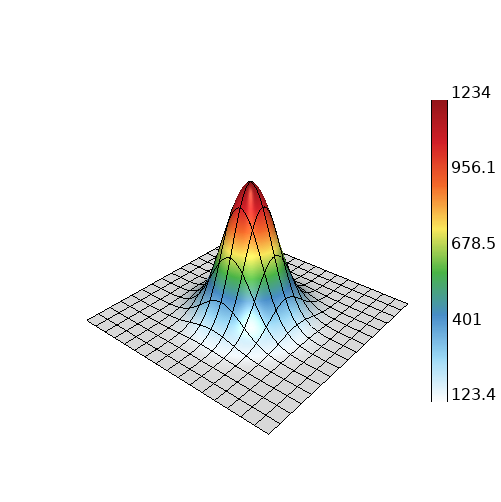
\includegraphics[width=\fs\textwidth]{../figures/Rect_local_Te_3D_200.png}
&
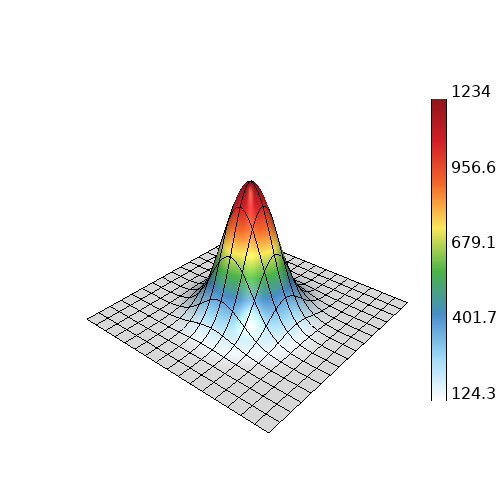
\includegraphics[width=\fs\textwidth]{../figures/Rect_local_Te_3D_50.png}
\end{tabular}
\end{center}
\end{frame}

\renewcommand{\fs}{0.35}
\begin{frame}
\begin{center}
%Local + nonlocal results, pAIR stats
\begin{tabular}{cc}
Local hydro temperature & Nonlocal kinetic temperature \\
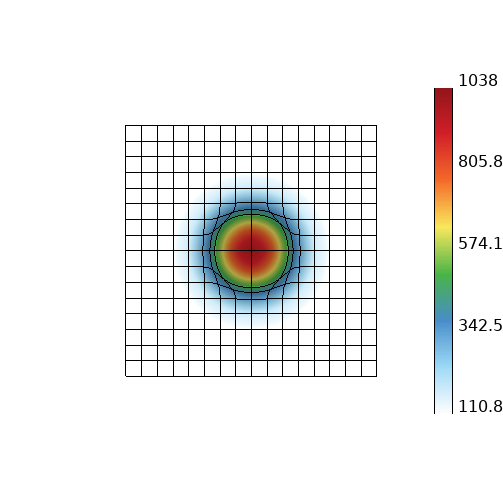
\includegraphics[width=\fs\textwidth]{../figures/ALE_local_Te_2D_neconst.png}
&
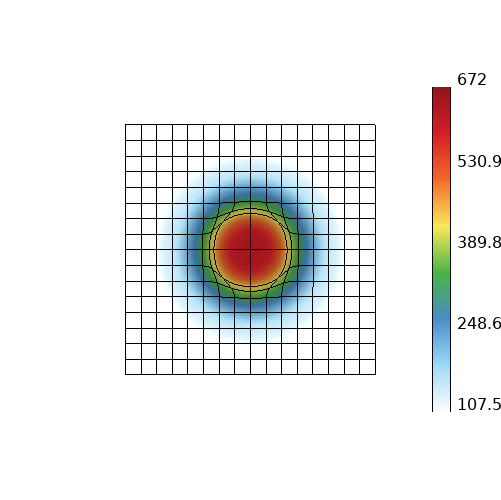
\includegraphics[width=\fs\textwidth]{../figures/ALE_nonlocal_Te_2D_neconst.png}
\\
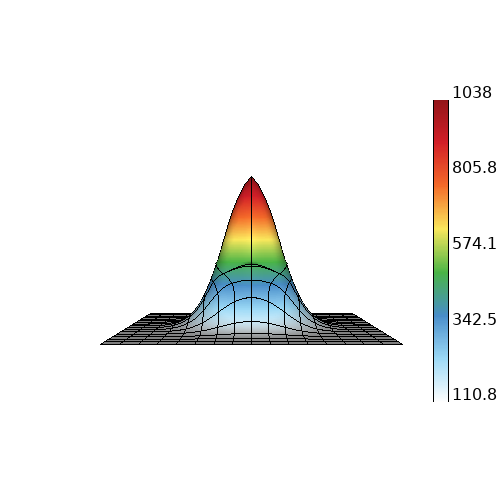
\includegraphics[width=\fs\textwidth]{../figures/ALE_local_Te_3D_neconst.png}
&
    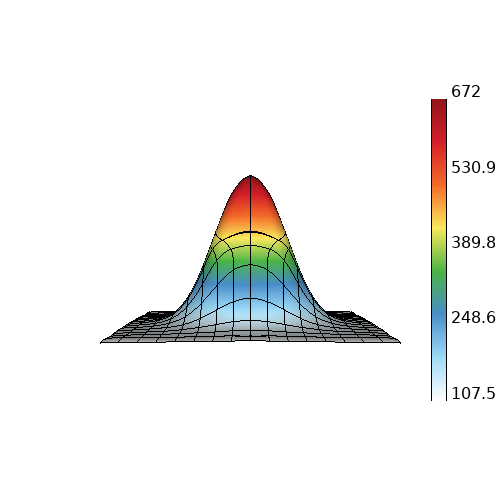
\includegraphics[width=\fs\textwidth]{../figures/ALE_nonlocal_Te_3D_neconst.png}
\end{tabular}
\end{center}
\end{frame}

\section{P$_N$ mixed finite element approach to kinetics}
\newcommand{\edf}{\colorimportant{f}}
\renewcommand{\fs}{0.4}
\begin{frame}
\begin{center}
%{\huge Nonlocal electron transport regime - PIC/VFP0/AWBS}
{\Large AP1 High-Order Mixed FEM formulation, fixed P1 angular discretization PCG(AMG)}
\begin{eqnarray}
  \matr{M}^{L_2}_{_{(\tilde{\nue})}}\cdot\ddv{\vfzero}{\vmag} 
  - \matr{V}^{L_2}_{_{(\frac{\xi\qe\E}{\me\vmag})}}\cdot\ddv{\fone}{\vmag}
  &=&
  \matr{D}^{L_2}_{_{(\xi)}}\cdot\fone 
  + \matr{M}^{L_2}_{_{(\frac{\xi2\qe\E}{\me\vmag^2})}}\cdot\fone
  + \vect{S}^{L_2}_{_{(\tilde{\nue}\pdv{\fM}{\vmag})}}, 
  \nonumber\label{eq:FEMAP1f0}
  \\
  \matr{M}^{H_1}_{_{(\tilde{\nue})}}\cdot\ddv{\fone}{\vmag}
  - \matr{V}^{H_1}_{_{(\frac{\qe\E}{\me\vmag})}}\cdot\ddv{\vfzero}{\vmag}
   &=& 
  \matr{G}^{H_1}\cdot\vfzero 
  + \matr{M}^{H_1}_{_{(\frac{\nuscat}{\vmag})}}\cdot\fone 
  + \matr{C}^{H_1}_{_{(\frac{\qe\B}{\me c \vmag}\vect{\times})}}\cdot\fone
  ,
  \nonumber \label{eq:FEMAP1f1}
\end{eqnarray}

\begin{tabular}{c}
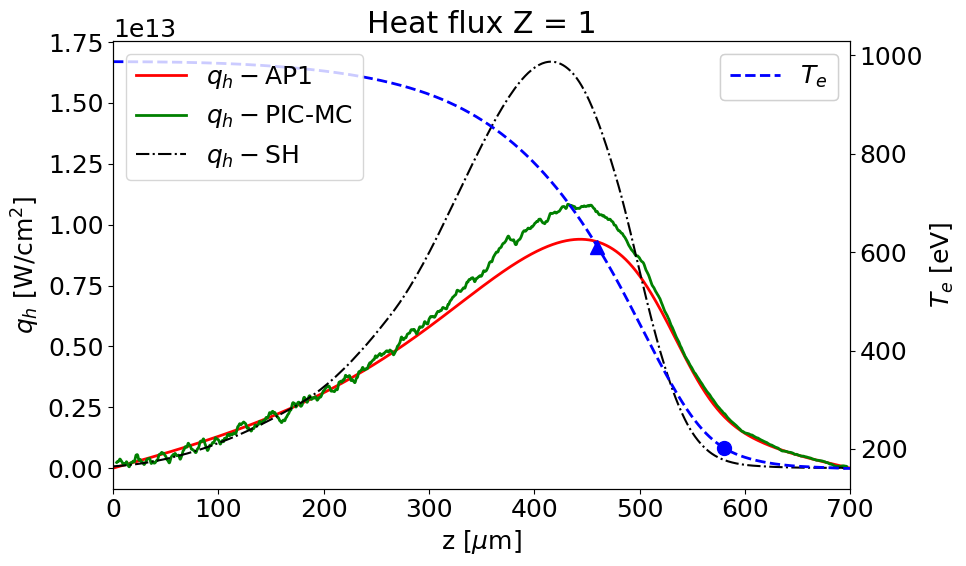
\includegraphics[width=\fs\textwidth]{../figures/C7_Calder_case5_heatflux_noSNB.png}
\end{tabular}
\begin{tabular}{cc}
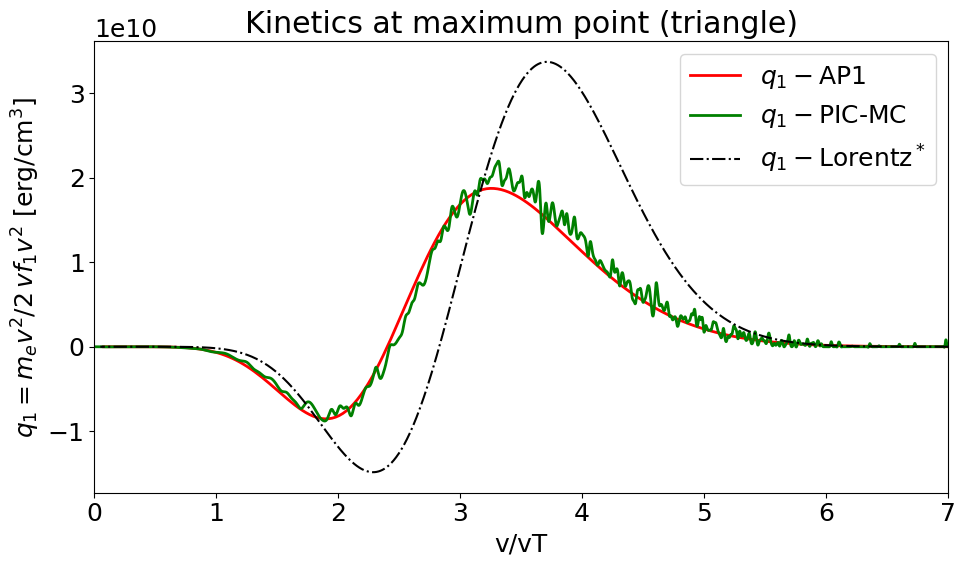
\includegraphics[width=\fs\textwidth]{../figures/C7_Calder_case5_kinetics_noSNB.png}
&
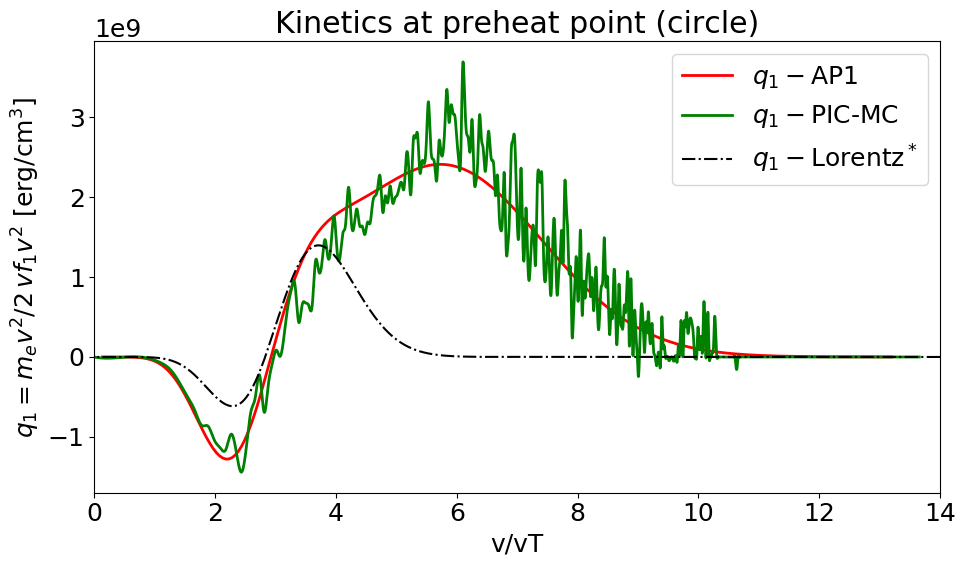
\includegraphics[width=\fs\textwidth]{../figures/C7_Calder_case5_nonlocal_kinetics_noSNB.png}
\end{tabular}
\let\thefootnote\relax\footnote{M. Holec et al, \textit{Phys. Plas.}, submitted (2019) / arXiv:1901.11378 .}
\end{center}
\end{frame}

\section{Conclusions}

\begin{frame}
\begin{center}
{\Large Electron velocity limit - friction vs. $\vect{E}$ stopping}
\begin{equation}
  \left( \tilde{\nue} - \frac{\E\cdot\vn}{\vmag} \right) 
  \frac{\partial f}{\partial \vmag}
  =
  \vn\cdot\nabla f 
  + \frac{\nuscat}{\vmag} \left(f - \fzero\right)
  + \frac{E_\phi 
  - \vmag~B_\theta}{\vmag^2}\pdv{f}{\phi}
  + \frac{E_\theta + \vmag~B_\phi}{\vmag^2\sin(\phi)}\pdv{f}{\theta}
  + \tilde{\nue} \frac{\partial \fM}{\partial v} .
  \nonumber
\end{equation}

\begin{tabular}{c}
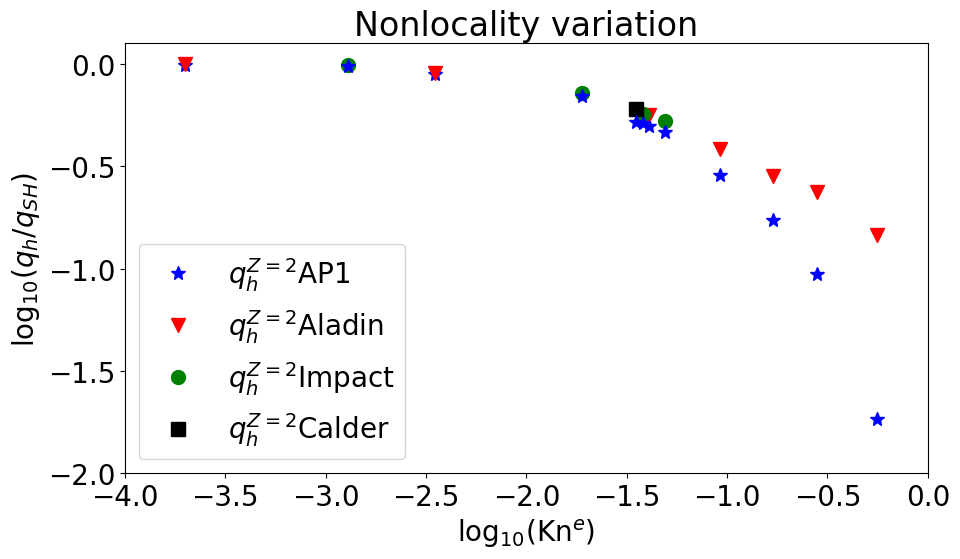
\includegraphics[width=0.5\textwidth]{../figures/Kn_results.png}
\end{tabular}

$\vect{E}$ stopping overtakes collisions for Kn$~>0.1$ .
\let\thefootnote\relax\footnote{M. Holec et al, \textit{Phys. Plas.}, submitted (2019) / arXiv:1901.11378 .}

\begin{tabular}{c|ccccc}
    \hline\hline\\
    %Kn$^e$ & $10^{-4}$ & $10^{-3}$ & $10^{-2}$ & $10^{-1}$ & $1$ \\\\
    Kn = $\frac{\lambda}{L}$ & $\,\,10^{-4}\,\,$ & $\,\,10^{-3}\,\,$ & $\,\,10^{-2}\,\,$ & $\,\,10^{-1}\,\,$ & $\,\,1\,\,$ \\\\
    \hline\\
    $v_{lim} / v_{th}$ & 70.8 & 22.4 & 7.3 & 3.1 & 1.8\\\\
    \hline\hline
\end{tabular} 
\end{center}
\end{frame}

\begin{frame}
\begin{center}
{\Large Adaptive DSA preconditioner for Hydro-Kinetics coupling}
\begin{myNblock}{AWBS electron kinetic model 7D}
\begin{eqnarray}
  C_V \frac{\dI T_e}{\dI t} 
  %&=& 
  %- \nabla\cdot\vect{q}_e(f) 
  %+ \vect{j}(f)\cdot\E
  %+ S_H , 
  %\nonumber \\
  &=& 
    \int_{\vect{v}} \sigma K(f)\dI\vect{v} - \sigma \Te^\alpha , 
  \nonumber \\
  \vect{v}\cdot\nabla f +
  \left( \vect{E} + \vect{v}\times\vect{B}\right)\cdot\nabla_{\vect{v}} f
  &=& 
  v \tilde{\nue} \frac{\partial }{\partial v}\left(f - f_{MB}(T_e)\right)
  + \nuscat \left(\fzero - f \right) .
  \nonumber
\end{eqnarray}
\end{myNblock}
Continuum analysis of local (Kn$\ll$1) transport regime $\rightarrow$ DIFFUSION
\begin{equation}
  C_V \frac{\dI T_e}{\dI t}
  = \nabla \cdot \lambda(\Te^{2.5}) \nabla \Te + O(\text{Kn}^2)
  \nonumber
\end{equation}
\begin{myNblock}{Precodnitioned fixed-point iteration $\matr{E}(\Delta \vect{T})\equiv(\matr{I} - \matr{C})\cdot\matr{M}_{\sigma}(\tilde{\vect{T}} + \Delta\vect{T})^\alpha - \matr{C}\cdot\matr{D}_{\lambda}(\tilde{\vect{T}} + \Delta\vect{T})^\alpha$}
%\begin{myNblock}{ $\matr{E}(\Delta \vect{T}) (\matr{I} - \matr{C})\cdot\matr{M}_{\sigma} + \matr{C}\cdot\matr{D}_{\lambda}$ }
\begin{equation}
\matr{M}_{C_V}\cdot\frac{\Delta \vect{T}^{k+1}}{\Delta t} + \matr{E}(\Delta \vect{T}^{k+1}) - \matr{E}(\Delta \vect{T}^{k}) = \matr{K}_\sigma (f^k) - \matr{M}_{\sigma}(\tilde{\vect{T}} + \Delta\vect{T}^k)^\alpha .
  \nonumber
\end{equation}
\end{myNblock}
Finally, we get an unconditionally stable backward Euler (SDIRK) fast iterating scheme
\begin{equation}
  \matr{M}_{C_V}\cdot\frac{\Delta \vect{T}^{k+1}}{\Delta t}  
  + (\matr{I} - \matr{C})\cdot\matr{M}_{\sigma}(\tilde{\vect{T}} + \Delta\vect{T}^{k+1})^\alpha - \matr{C}\cdot\matr{D}_{\lambda}(\tilde{\vect{T}} + \Delta\vect{T}^{k+1})^\alpha
  =   
  \matr{K}(f^k) - \matr{C}\cdot\matr{M}_{\sigma}(\tilde{\vect{T}} + \Delta\vect{T}^k)^\alpha - \matr{C}\cdot\matr{D}_{\lambda}(\tilde{\vect{T}} + \Delta\vect{T}^{k})^\alpha,  \nonumber
\end{equation}
where adaptive coefficient diffusion $\matr{C}\xrightarrow{\text{Kn}\ll1} 1$ and nonlocal transport $\matr{C}\xrightarrow{\text{Kn}>1} 0$ and $\matr{C}\in (1, 0)$ in between.
{\small T. Haut et al, \textit{SIAM}, submitted (2018) / arXiv:1810.11082 .}
\end{center}
\end{frame}

\begin{frame}
\begin{center}
{\huge Conclusions}
\begin{itemize}
  \item 7D microscopic world of electrons in hydro simulations.
  \item S$_N$ high-order DG finite element approach.
  \item P$_1$ high-order mixed finite element approach.
  \item $\E$ field dominated stopping (P$_1$ fails).
  \item Adaptive DSA preconditioner for Hydro-Kinetics coupling (ML on $\matr{C}$).
  \item Algebraic Multigrid solver pAIR scales $\log(P)^{1.22}$.
\end{itemize}
\begin{tabular}{lll}
%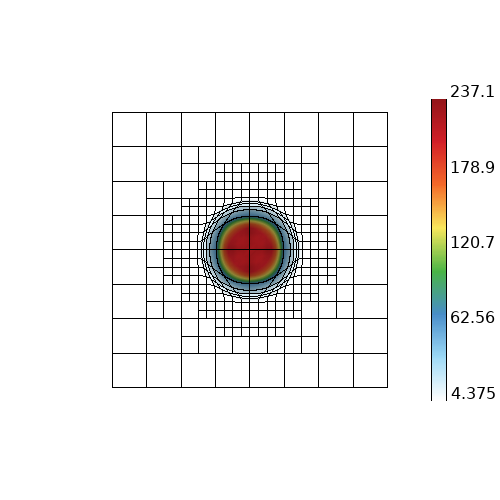
\includegraphics[width=0.3\textwidth]{../figures/AMR_ALE_nonlocal_Te_2D.png} &
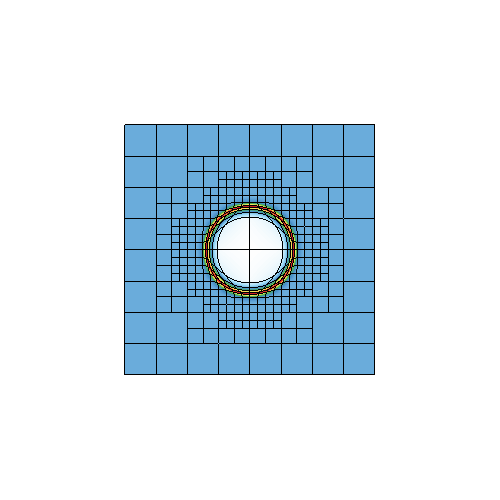
\includegraphics[width=0.3\textwidth]{../figures/AMR_ALE_density_2D_nobar.png} &
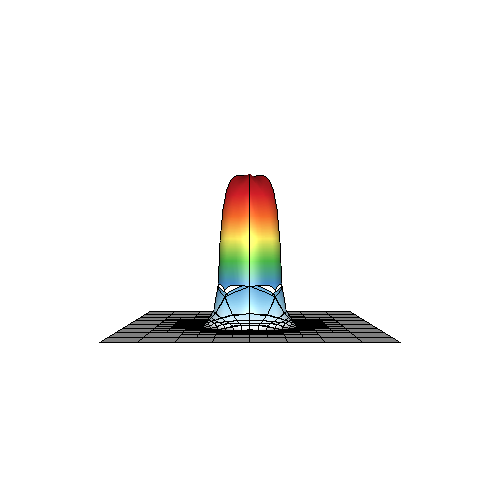
\includegraphics[width=0.3\textwidth]{../figures/AMR_ALE_nonlocal_Te_3D_nobar.png} &
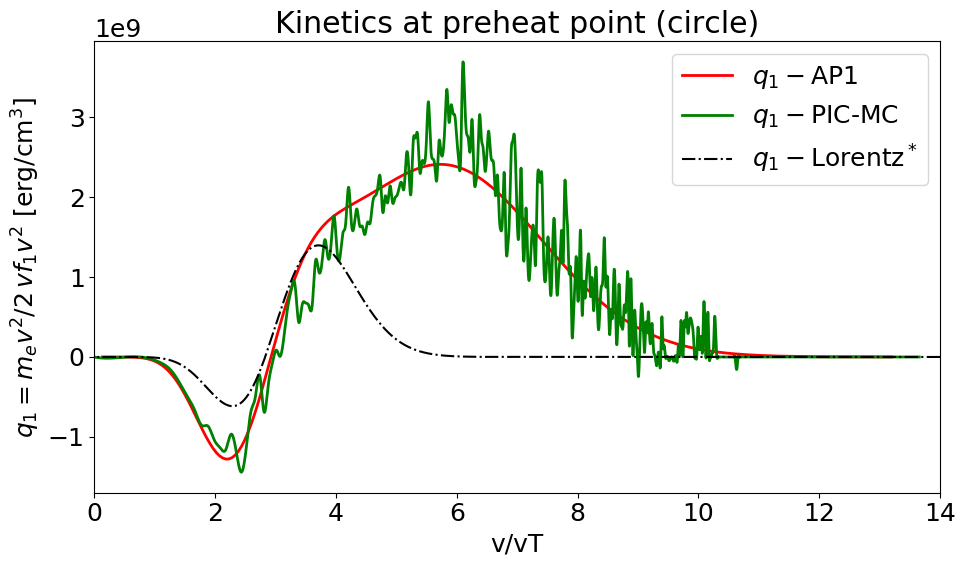
\includegraphics[width=0.4\textwidth]{../figures/C7_Calder_case5_nonlocal_kinetics_noSNB.png}
%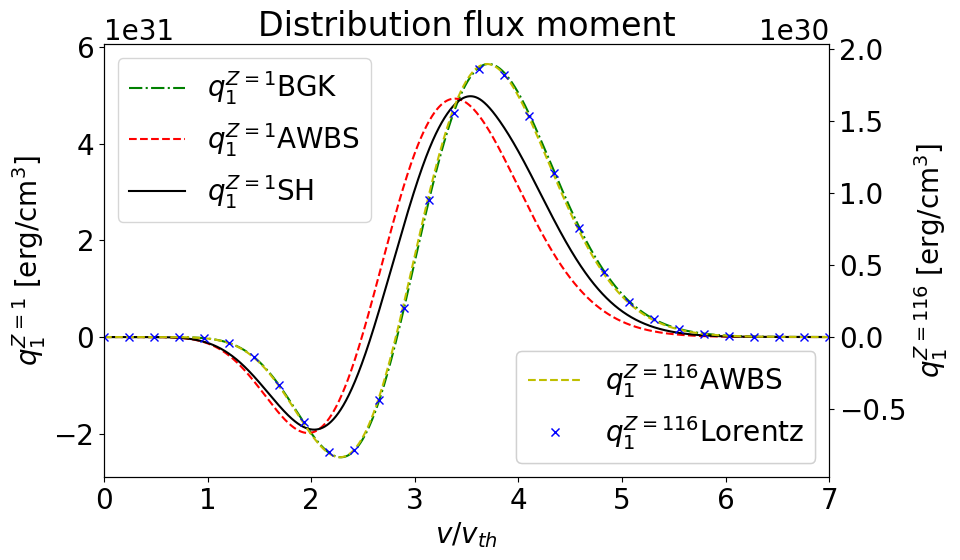
\includegraphics[width=0.3\textwidth]{../figures/q1s.png} &
%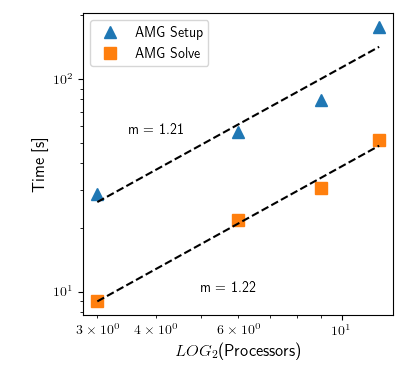
\includegraphics[width=0.3\textwidth]{../figures/pAIR_scaling.png}
\end{tabular}
\let\thefootnote\relax\footnote{MS85 - Developments in Algebraic Multigrid for Nonsymmetric and Hyperbolic Problems - Ben S. Southworth}
\let\thefootnote\relax\footnote{https://github.com/CEED/Laghos/tree/master/amr}
\let\thefootnote\relax\footnote{https://mfem.org}
\end{center}
\begin{tabular}{l}
\hline\\
MS85 - Developments in Algebraic Multigrid for Nonsymmetric and Hyperbolic Problems - Ben S. Southworth \\
https://github.com/CEED/Laghos/tree/master/amr \\
https://mfem.org \\
\textit{holec1@llnl.gov}
\end{tabular}
\end{frame}

\begin{frame}
  \begin{textblock}{16}(0,6)
    \centering
      {\color{white}\bf {\huge Thank you for your attention. Any questions?}}
  \end{textblock}


  \tikz[overlay,remember picture] 
\node[scale=0.6,text width=5in,  at=(current page.south east), anchor=south east,inner sep=0pt] at (330pt,-150pt) {\color{white}  Disclaimer: This document was prepared as an account of work sponsor bt an agency of the United States government, Neither the United States government or Lawrence Livermore Nation Security, LLC, nor any of their employees make any warranty, expressed or implied, or assumes any legal liability or responsibility for the accuracy, completeness, or usefulness of any information, apparatus, product, or process disclosed, or represent that its use would not infringe privately owned rights. Reference herein to any specific commercial product, process, or service by trade name, trademark, manufacturer, or otherwise does not necessarily constitute or imply its endorsement, recommendation, or favoring by the United States government or Lawrence Livermore National Security, LLC. The views and options of authors expressed herein do not necessarily state or reflect those of the United States government or Lawrence Livermore Nation Security, LLC, and shall not be used for advertising or product endorsement purposes. };


\end{frame}

\begin{comment} % Nonlocal Ohm
\begin{frame}
\begin{center}
{\Large Nonlocal Ohm's law}

We found that the~quality of the~electric field evaluation is essential for 
a~correct plasma modeling 
\begin{block}{Nonlocal current in plasma}
\begin{equation}
  \vect{j}(f, \vect{E}) = e \int v \fone v^2~\dI v = 
  e \int v \frac{\nuei^2 \vect{E}^* 
  + \omegaB~\omegaB\cdot\vect{E}^* + \nuei~\omegaB \times \vect{E}^*}
  {\nuei (\omegaB^2 + \nuei^2)} v^2~\dI v ,
  \label{eq:NonlocalOhm}
\end{equation}
\end{block}
where $\vect{E}^* = \vmag\frac{\nue}{2}\pdv{\fone}{\vmag} 
- \vmag\nabla\cdot\matr{f}_2 
 - \frac{\qe}{\me}\E\pdv{\fzero}{\vmag}$ 
is an effective electric field in plasma. 
A~comparison to the \textit{Generalized Ohm's law} shows a~correct local 
behavior of \eqref{eq:NonlocalOhm}, especially that 
$\nabla\times \nabla\cdot\matr{f}_2 
\sim \nabla\times \frac{\nabla p_e}{\ed} \sim \nabla n_e \times \nabla T_e$

\begin{block}{Generalized Ohm's law vs. nonlocal Ohm's law}
\begin{eqnarray} 
  \vect{E} &=&  
  \left(\vect{R}_T -\nabla p_e\right)\quad + ~~~~~\quad\qquad 
  \frac{\vect{j}}{\sigma}\qquad\quad ~~~~+
  \qquad \vect{j}\times\vect{B} ,
  \nonumber \\
  \vect{E} \vmag \frac{\qe}{\me}\pdv{\fzero}{\vmag} 
  &=& 
  ~~~~\vmag^2 \nabla\cdot\matr{f}_2 ~~~~~~ 
  +~~~  \vmag^2 \frac{\nue}{2}\pdv{\fone}{\vmag} - \vmag \nuei\fone 
  ~~~+~~~ v \fone\times\frac{\qe}{\me c}\vect{B}.
  %\vect{E} \int v \pdv{\fzero}{v} v^2\, \dI v 
  %&=& 
  %\int v^2 \nabla \fzero v^2\, \dI v~~~ +~~  \int v \nuei\fone v^2\, \dI v 
  %~~~+~~ \int v \fone\times\vect{B} v^2\, \dI v .
  \nonumber
\end{eqnarray}
\end{block}

\end{center}
\end{frame}
\end{comment} % Nonlocal Ohm

\end{document}
